
\section{Dữ liệu 4}
Bộ dữ liệu ghi lại những yếu tố có thể ảnh hưởng đến lương (\$ giờ) của người lao động ở Anh năm 1976

\subsection*{Tìm hiểu dữ liệu}
Bộ dữ liệu gồm 13 biến sau:
\begin{itemize}
	\item \texttt{wage}: Số lượng trung bình một giờ
	\item \texttt{educ}: Số năm học
	\item 
\end{itemize}

\subsection*{Phân tích dữ liệu}

Dựa vào độ tương quan ta nhận thấy được ba biến \texttt{lwage}, \texttt{tenursq}, \texttt{expersq} trên 90 nên ta sẽ bỏ ba biến này ra khỏi bộ dữ liệu
Nên ta sẽ tiến hành kiểm định thử xem ta có thể bỏ được 3 biến này được hay không

\subsection*{Chọn mô hình}
\subsubsection*{Hướng tiếp cận 1: Chọn tất cả}

% Please add the following required packages to your document preamble:
% \usepackage{longtable}
% Note: It may be necessary to compile the document several times to get a multi-page table to line up properly
\begin{longtable}{clllll}
	\hline
	\begin{tabular}[c]{@{}c@{}}Số lượng \\ biến\end{tabular} &
	\multicolumn{1}{c}{Biến dự đoán} &
	\multicolumn{1}{c}{R\textasciicircum{}2} &
	\multicolumn{1}{c}{AIC} &
	\multicolumn{1}{c}{Cp} &
	\multicolumn{1}{c}{BIC} \\ \hline
	\endhead
	%
	\hline
	\endfoot
	%
	\endlastfoot
	%
	1 &
	profocc &
	\multicolumn{1}{c}{0.19362} &
	\multicolumn{1}{c}{} &
	243.45475 &
	-101.6706 \\
	2 &
	educ, tenure &
	\multicolumn{1}{c}{0.29919} &
	\multicolumn{1}{c}{} &
	143.97580 &
	-170.2154 \\
	3 &
	educ, tenure, female &
	\multicolumn{1}{c}{0.35396} &
	\multicolumn{1}{c}{} &
	92.91189 &
	-207.7622 \\
	4 &
	educ, tenure, female, profocc &
	0.39249 &
	&
	57.37900 &
	-234.8483 \\
	5 &
	educ, tenure, femanle, profocc, trade &
	0.41818 &
	&
	34.07821 &
	-252.3208 \\
	6 &
	educ, tenure, female, profocc, trade, west &
	0.42657 &
	&
	27.14121 &
	-254.7032 \\
	7 &
	educ, tenure, female, profocc, trade, west,  services &
	0.43425 &
	&
	20.89218 &
	-256.5481 \\
	8 &
	educ, tenure, female, profocc, trade, west, services, smsa &
	0.44033 &
	&
	16.16804 &
	-256.9875 \\
	9 &
	educ, tenure, female, profocc, trade, west, services, smsa, married &
	0.44469 &
	&
	13.08489 &
	-255.8480 \\
	10 &
	educ, tenure, female, profocc, trade, west, services, smsa, married, northcen &
	0.44560 &
	&
	13.22747 &
	-251.4683 \\
	11 &
	\begin{tabular}[c]{@{}l@{}}educ, tenure, female, profocc, trade, west, services, smsa, \\ married, ndurman, profserv\end{tabular} &
	0.44637 &
	&
	13.50318 &
	-246.9594 \\
	12 &
	\begin{tabular}[c]{@{}l@{}}educ, tenure, female, profocc, trade, west, services, smsa, \\ married, ndurman, profserv, trcommpu\end{tabular} &
	0.44827 &
	&
	12.73335 &
	-243.5280 \\
	13 &
	\begin{tabular}[c]{@{}l@{}}educ, tenure, female, profocc, trade, west, services, smsa, \\ married, ndurman, profserv, trcommpu, northcen\end{tabular} &
	0.44939 &
	&
	12.69999 &
	-239.3528 \\
	14 &
	\begin{tabular}[c]{@{}l@{}}educ, tenure, female, profocc, trade, west, services, smsa, \\ married, ndurman, profserv, trcommpu, northcen, numdep\end{tabular} &
	0.44959 &
	&
	13.51543 &
	-234.3090 \\
	15 &
	\begin{tabular}[c]{@{}l@{}}educ, tenure, female, profocc, trade, west, services, smsa, \\ married, ndurman, profserv, trcommpu, northcen, numdep, exper\end{tabular} &
	0.45032 &
	&
	13.84069 &
	-229.7754 \\
	16 &
	\begin{tabular}[c]{@{}l@{}}educ, tenure, female, profocc, trade, west, services, smsa, married, ndurman, \\ profserv, trcommpu, nothcen, numdep, exper, south\end{tabular} &
	0.45015 &
	&
	15.00327 &
	-224.3782 \\
	17 &
	\begin{tabular}[c]{@{}l@{}}educ, tenure, female, profocc, trade, west, services, smsa, married, ndurman,\\  profserv, trcommpu, northcen, numdep, exper, construc, clerocc\end{tabular} &
	0.45003 &
	&
	16.12009 &
	-219.0300 \\
	18 &
	\begin{tabular}[c]{@{}l@{}}educ, tenire, female, profocc, trade, west, services, smsa, married, ndurman, \\ profserv, trcommpu, northcen, numdep, exper, construc, clerocc, south\end{tabular} &
	0.44988 &
	&
	17.26616 &
	-213.6529 \\
	19 &
	\begin{tabular}[c]{@{}l@{}}educ, tenire, female, profocc, trade, west, services, smsa, married, ndurman, \\ profserv, trcommpu, northcen, numdep, exper, construc, clerocc, south, servocc\end{tabular} &
	0.44906 &
	&
	19.01455 &
	-207.6496 \\
	20 &
	\begin{tabular}[c]{@{}l@{}}educ, tenire, female, profocc, trade, west, services, smsa, married, ndurman, profserv, \\ trcommpu, northcen, numdep, exper, construc, clerocc, south, servocc, nonwhite\end{tabular} &
	0.44799 &
	&
	21.00000 &
	-201.3995 \\ \hline
\end{longtable}

Dựa vào bảng ta thấy được mô hình có chỉ số BIC tốt nhất là mô hình 8 biến. Tuy nhiên mô hình có hệ số xác định hiệu chỉnh tốt nhất là mô hình có 15 biến và mô hình có hệ số $C_p$ tốt nhất là mô hình 19 biến dự đoán

\subsubsection*{Hướng tiếp cận 2: Phương pháp tiến dựa trên AIC}

\lstinputlisting[float=h,frame=tb,caption=R output,label=zebra]{../Output Of R/StepAIC_back.txt}

Sau khi chạy code R phương pháp lùi dựa theo tiêu chí AIC thì mô hình chọn được là mô hình gồm 11 biến
\[\texttt{wage} = \texttt{educ} + \beta_0\texttt{tenure} + \texttt{female} + married + smsa + northcen + west + ndurman + trcommpu + trade + services + profserv + profocc\]

\subsubsection*{Hướng tiếp cận 3: Phương pháp Stagewise}
\begin{figure}[]
	\centering
	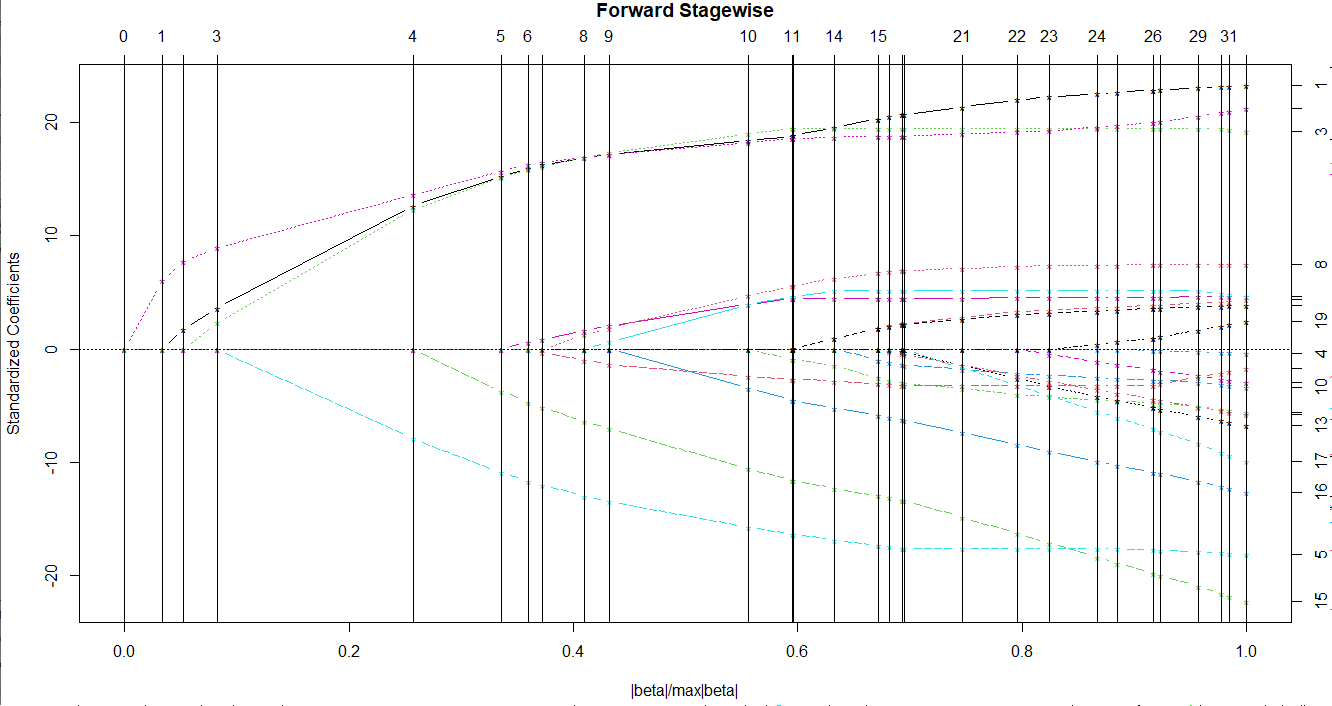
\includegraphics[width=.85\linewidth]{../Photo Of Result/stagewise plot}
\end{figure}

Dựa vào hình và bảng trên phương pháp Stagewise đưa ra đề xuất model gồm 11 biến
\[\texttt{wage} = \texttt{educ} + \texttt{tenure} + \texttt{female} + \texttt{married} + \texttt{smsa} + \texttt{west} + \texttt{trade} + \texttt{services} + \texttt{profocc} + \texttt{servocc} \]

Dựa vào cả ba hướng tiếp cận, ta sẽ xây dựng 5 mô hình hồi quy lại theo các phương pháp chọn biến


Dựa vào kết quả hồi quy của R chạy thì ta chọn mô hình 8 biến theo phương pháp chọn tất cả dựa vào chuẩn BIC. Tuy nhiên, các hệ số hồi quy vẫn chưa đạt được mức ý nghĩa thống kê nên ta tiến hành lấy log để xem thử


